\section{Statistics for Beginner's Algorithm}
\label{sec:beginnersStat}
In order to get the average length of a solution of Beginner's algorithm we must determine how many moves of scrambling must be applied in order to find the worst case scenario. 
By computing the average for different amount of scrambles the graph quickly becomes steady at around 40 scrambles (10.000 cubes is tested). See figure \ref{fig:beginnersScramble}. To be sure that we get a good result we go by 50 scrambles.
\begin{figure}[htbp]
	\centering
		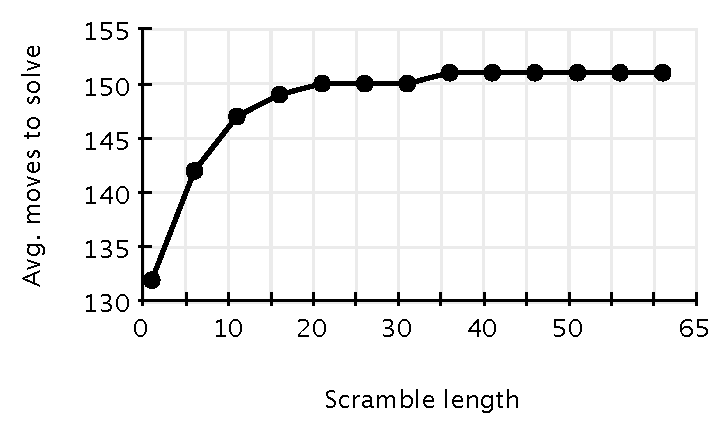
\includegraphics{input/pics/beginnersScramble.pdf}
	\caption{\myCaption{The graph shows the amount of moves needed to solve a cube with x scrambles. The lines are for showing only and do not represent the average between the dots.}}
	\label{fig:beginnersScramble}
\end{figure}

Now that the number of scrambles is determined the average can be found.
By scrambling 1.000.000 cubes and solve them with the beginner's algorithm we get an average of 151 moves. 
Which is the average of beginner's algorithm. The test were run 3 times all with same results.
The maximum value found is 224 moves and minimum is 70 moves. The time were XXXX minutes. 
The data was gathered on a 2.5 GHz AMD Quad Core processor (905e) with 4 GB DDR-3 RAM running on Windows 7 64 bits.

A peculiar note is that with one twist, the algorithm needs an average of 131 moves with a maximum of 155 and a minimum 94 moves to solve it again.
This illustrates the twist-wise inefficiency of this algorithm very well.


